\documentclass{ntuabeamer}
\usepackage{appendixnumberbeamer}
\usepackage[utf8]{inputenc}
\usepackage{amsmath,amssymb,tikz}
\usetikzlibrary{arrows.meta,calc,positioning}
\usepackage{pgfplots}
\pgfplotsset{compat=1.18}

\framesource{kipf2017}{Kipf, Welling. \emph{Semi-Supervised Classification with Graph Convolutional Networks}. ICLR, 2017.}
\framesource{hamilton2017}{Hamilton, Ying, Leskovec. \emph{Inductive Representation Learning on Large Graphs}. NeurIPS, 2017.}
\framesource{velickovic2018}{Veli\v{c}kovi\'{c} et al. \emph{Graph Attention Networks}. ICLR, 2018.}
\framesource{xu2019}{Xu et al. \emph{How Powerful are Graph Neural Networks?} ICLR, 2019.}

\title{Graph Neural Networks}
\author{}
\date{}

\definecolor{courseblue}{HTML}{3F7CAC}
\definecolor{courseorange}{HTML}{D97706}
\definecolor{coursegreen}{HTML}{27864A}
\definecolor{coursegray}{HTML}{667085}
\definecolor{coursepurple}{HTML}{7656A3}
\definecolor{coursered}{HTML}{B5473C}
\definecolor{courselightblue}{HTML}{DCE9F5}
\definecolor{courselightorange}{HTML}{F9E4C8}
\newcommand{\takeaway}[1]{\par\medskip{\raggedright\color{courseblue}\bfseries #1\par}}

\tikzset{
  flow/.style={-{Latex[length=3mm]},very thick,courseblue},
  edge/.style={very thick,coursegray},
  focus/.style={very thick,courseorange},
  vertex/.style={circle,draw,very thick,minimum size=0.8cm,inner sep=0pt,fill=courselightblue},
  box/.style={draw,rounded corners,very thick,align=center,minimum width=1.7cm,minimum height=0.85cm}
}

% The five-node example graph used throughout: #1 styles node 1; #2..#6 are the node contents.
\newcommand{\examplegraph}[6][]{%
  \node[vertex,font=\footnotesize,#1] (a) at (0,0) {#2};
  \node[vertex,font=\footnotesize] (b) at (2,1.4) {#3};
  \node[vertex,font=\footnotesize] (c) at (4.3,0.5) {#4};
  \node[vertex,font=\footnotesize] (d) at (1.6,-1.5) {#5};
  \node[vertex,font=\footnotesize] (e) at (4.5,-1.6) {#6};
  \draw[edge] (a)--(b)--(c)--(e)--(d)--(a);
  \draw[edge] (b)--(d); \draw[edge] (c)--(d);%
}

\begin{document}
\begin{frame}[plain]\makepresentationtitle\end{frame}



\section{Graphs and Their Data}
\sectiondivider{Graphs and Their Data}

\begin{frame}{Graphs Represent Irregular Relations}
  Images live on a regular grid and sequences on a line. Many engineering objects do not:
  structures, meshes, molecules, road networks, social networks.
  \begin{center}
  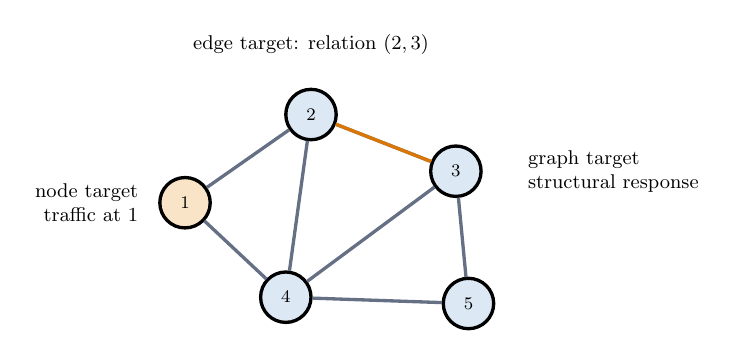
\begin{tikzpicture}[scale=0.8,transform shape]
    \examplegraph[fill=courselightorange]{$1$}{$2$}{$3$}{$4$}{$5$}
    \node[left=0.2cm of a,align=right,font=\small] {node target\\traffic at 1};
    \node[above=0.4cm of b,font=\small] {edge target: relation $(2,3)$};
    \draw[focus] (b)--(c);
    \node[right=0.6cm of c,align=left,font=\small] {graph target\\structural response};
  \end{tikzpicture}
  \end{center}
  \takeaway{Variable neighborhoods and meaningful relations call for a graph.}
\end{frame}

\begin{frame}{Graph Data: Nodes, Edges, Features}
  A graph $G=(V,E)$ has a set $V$ of $N$ nodes and a set $E$ of edges.
  Information is attached at three levels:
  \begin{itemize}
    \item node features $\mathbf x_v\in\mathbb R^{d_x}$ (for example a load or a material),
    \item edge features $\mathbf e_{uv}\in\mathbb R^{d_e}$ (for example a length),
    \item global features $\mathbf u\in\mathbb R^{d_u}$ (for example temperature).
  \end{itemize}
  Stacking the node features as rows gives $\mathbf X\in\mathbb R^{N\times d_x}$.
  The \emph{neighborhood} $\mathcal N(v)$ is the set of nodes with an edge into $v$.
  \takeaway{So a graph dataset is: who is connected to whom, plus feature vectors on nodes, edges and the whole graph.}
\end{frame}

\begin{frame}{The Adjacency Matrix Stores Who Is Connected}
  The \emph{adjacency matrix} $\mathbf A\in\{0,1\}^{N\times N}$ has $A_{vu}=1$ when there is an edge between $v$ and $u$.
  For the five-node graph (rows and columns in order $1,\dots,5$):
  \[
    \mathbf A=\begin{bmatrix}
      0&1&0&1&0\\
      1&0&1&1&0\\
      0&1&0&1&1\\
      1&1&1&0&1\\
      0&0&1&1&0
    \end{bmatrix}
  \]
  Row 1 reads: node 1 is connected to nodes 2 and 4, so $\mathcal N(1)=\{2,4\}$.
  This graph is undirected, so $\mathbf A=\mathbf A^{\mathsf T}$.
  \takeaway{So $\mathbf A$ is the graph written as a table, and each row lists one node's neighbors.}
\end{frame}





\section{Node Labels Must Not Matter}
\sectiondivider{Node Labels Must Not Matter}

\begin{frame}{Node Labels Are Arbitrary}
  \begin{center}
  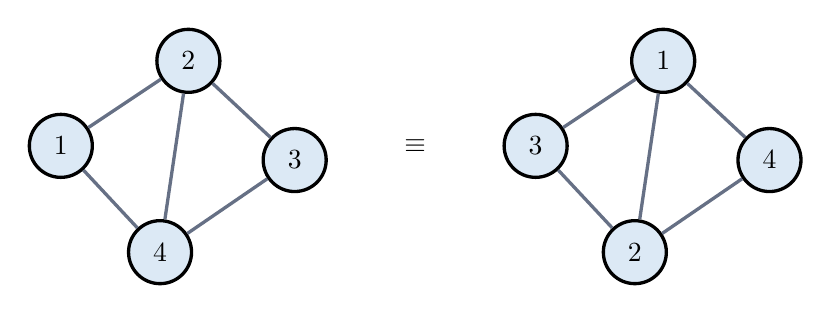
\begin{tikzpicture}[scale=0.9]
    \node[vertex] (a1) at (0,0) {$1$}; \node[vertex] (a2) at (1.8,1.2) {$2$};
    \node[vertex] (a3) at (3.3,-0.2) {$3$}; \node[vertex] (a4) at (1.4,-1.5) {$4$};
    \draw[edge] (a1)--(a2)--(a3)--(a4)--(a1); \draw[edge] (a2)--(a4);
    \node at (5.0,0) {$\equiv$};
    \node[vertex] (b1) at (6.7,0) {$3$}; \node[vertex] (b2) at (8.5,1.2) {$1$};
    \node[vertex] (b3) at (10,-0.2) {$4$}; \node[vertex] (b4) at (8.1,-1.5) {$2$};
    \draw[edge] (b1)--(b2)--(b3)--(b4)--(b1); \draw[edge] (b2)--(b4);
  \end{tikzpicture}
  \end{center}
  Both drawings are the same graph with the nodes numbered differently. In arrays, renumbering
  reorders the rows of $\mathbf X$ and the rows and columns of $\mathbf A$:
  $\mathbf X'=\mathbf P\mathbf X$, $\mathbf A'=\mathbf P\mathbf A\mathbf P^{\mathsf T}$,
  where $\mathbf P$ is a permutation matrix (it encodes the new numbering).
  \takeaway{So the numbering is a storage accident, and a sensible model must not depend on it.}
\end{frame}

\begin{frame}{Equivariance: Node Outputs Follow the Relabeling}
  A node-level model $F$ outputs one vector per node. Renumbering the input should renumber the output in the same way:
  \[
    \boxed{F(\mathbf P\mathbf X,\mathbf P\mathbf A\mathbf P^{\mathsf T})
      =\mathbf P F(\mathbf X,\mathbf A)}.
  \]
  \begin{itemize}
    \item Example: if the model predicts a load of $0.7$ at the node you called $3$, it must predict $0.7$ at that same node after you rename it $1$.
    \item This property is called \emph{permutation equivariance}.
  \end{itemize}
  \takeaway{So each node keeps its own prediction, wherever it is listed.}
\end{frame}

\begin{frame}{Invariance: Graph Outputs Ignore the Relabeling}
  A graph-level model $f$ outputs one answer for the whole graph, so renumbering should change nothing:
  \[
    \boxed{f(\mathbf P\mathbf X,\mathbf P\mathbf A\mathbf P^{\mathsf T})
      =f(\mathbf X,\mathbf A)}.
  \]
  \begin{itemize}
    \item Example: the sum of the node values $3,1,-1,2,-3$ is $2$ in any numbering.
    \item This property is called \emph{permutation invariance}.
    \item It is a required symmetry of the problem, not an optional data augmentation.
  \end{itemize}
  The geometric deep-learning lecture treats these symmetries in general.
  \takeaway{So graph predictions must be built from symmetric operations such as sums, means and maxima.}
\end{frame}



\section{Message Passing}
\sectiondivider{Message Passing}

\begin{frame}{Idea: Each Node Listens to Its Neighbors}
  A node knows only its own features. To understand its role it needs context, and its context is its neighbors.
  \emph{Message passing}: every node collects what its neighbors say and updates its own state.
  \begin{center}
  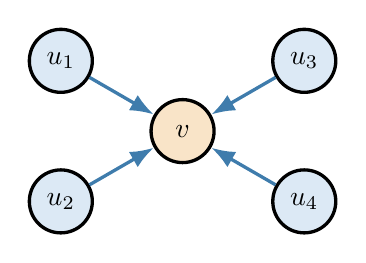
\begin{tikzpicture}[scale=0.85]
    \node[vertex,fill=courselightorange] (v) at (5,0) {$v$};
    \foreach \i/\ang in {1/150,2/210,3/30,4/-30}{
      \node[vertex] (n\i) at ($(v)+(\ang:2.1cm)$) {$u_{\i}$};
      \draw[flow] (n\i)--(v);
    }
  \end{tikzpicture}
  \end{center}
  \takeaway{So a node's new state is computed from its own state and from what its neighbors send.}
\end{frame}



\begin{frame}{Worked Example: One Layer on the Five-Node Graph}
  $\mathbf h^{(0)}=(3,1,-1,2,-3)$: send neighbor values, sum, then average with self.
  \begin{center}
  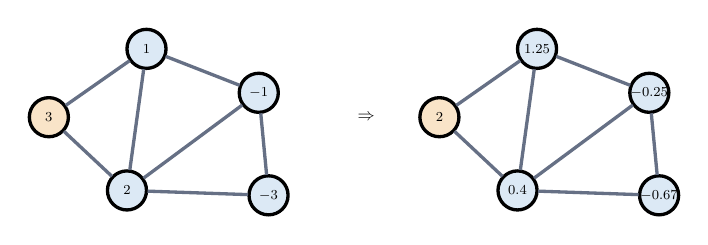
\begin{tikzpicture}[scale=0.62,transform shape]
    \examplegraph[fill=courselightorange]{$3$}{$1$}{$-1$}{$2$}{$-3$}
    \node at (6.5,0) {$\Rightarrow$};
    \begin{scope}[xshift=8cm]
      \examplegraph[fill=courselightorange]{$2$}{$1.25$}{$-0.25$}{$0.4$}{$-0.67$}
    \end{scope}
  \end{tikzpicture}
  \end{center}
  \begin{columns}[T]
    \begin{column}{0.29\textwidth}\centering\small
      \textbf{Message}\\[2mm]
      $m_{21}=1,\;m_{41}=2$
    \end{column}
    \begin{column}{0.35\textwidth}\centering\small
      \textbf{Aggregate}\\[2mm]
      $m_1=1+2=2+1=3$
    \end{column}
    \begin{column}{0.32\textwidth}\centering\small
      \textbf{Update}\\[2mm]
      $h_1^{(1)}=(3+3)/3=2$
    \end{column}
  \end{columns}
  \medskip
  {\small
  \[
    m_{uv}=M(\mathbf h_u,\mathbf h_v,\mathbf e_{uv}),\qquad
    \mathbf h_v^{(k+1)}=U\!\left(\mathbf h_v^{(k)},
       \operatorname{AGG}_{u\in\mathcal N(v)}m_{uv}\right).
  \]
  Shared $M,U$; sum, mean or max aggregation ignores neighbor order.}
\end{frame}



\begin{frame}{One Message-Passing Layer Is Permutation Equivariant}
  Renumber nodes with a permutation matrix $\mathbf P$. A layer $F$ satisfies
  \[
    \boxed{F(\mathbf P\mathbf H,\mathbf P\mathbf A\mathbf P^{\mathsf T})
      =\mathbf P F(\mathbf H,\mathbf A).}
  \]
  \begin{itemize}
    \item Shared messages use features, not node numbers.
    \item Sum, mean or max ignores neighbor order.
    \item Compatible equivariant layers compose.
  \end{itemize}
  Edge features, when present, must be relabeled with their endpoints.
  \takeaway{Relabel before or after the layer: the node outputs agree. Proof: appendix.}
\end{frame}

\begin{frame}{Depth Expands the Receptive Field by Graph Hops}
  \begin{center}
  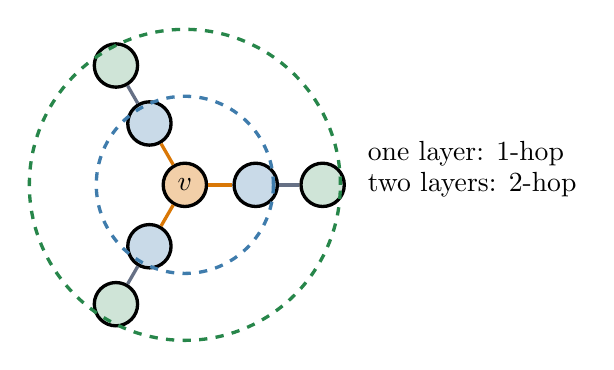
\begin{tikzpicture}[scale=0.5,vertex/.append style={minimum size=0.55cm}]
    \node[vertex,fill=courseorange!35] (v) at (0,0) {$v$};
    \foreach \i/\ang in {1/0,2/120,3/240}{
      \node[vertex,fill=courseblue!28] (a\i) at ($(v)+(\ang:1.8cm)$) {};
      \draw[focus] (v)--(a\i);
      \node[vertex,fill=coursegreen!22] (b\i) at ($(v)+(\ang:3.5cm)$) {};
      \draw[edge] (a\i)--(b\i);
    }
    \draw[courseblue,very thick,dashed] (v) circle (2.25cm);
    \draw[coursegreen,very thick,dashed] (v) circle (3.95cm);
    \node[right] at (4.4,0.8) {one layer: 1-hop};
    \node[right] at (4.4,0) {two layers: 2-hop};
  \end{tikzpicture}
  \end{center}
  After $k$ layers the state $\mathbf h_v^{(k)}$ depends on nodes at most $k$ hops (edges) away.
  In the five-node example, node 1 hears from nodes $2,4$ after one layer and from all five after two.
  \takeaway{So depth sets how far information travels: one hop per layer.}
\end{frame}



\section{Three Classic Layers: GCN, GraphSAGE, GAT}
\sectiondivider{Three Classic Layers: GCN, GraphSAGE, GAT}

\begin{frame}{GCN Idea: Average Neighbors, Corrected for Degree\framecite{kipf2017}}
  A plain sum over neighbors gives hub nodes (many neighbors) much larger values than leaves.
  The graph convolutional network (GCN) uses a degree-normalized sum:
  \begin{itemize}\small
    \item add a \emph{self-loop} so the node keeps its own state: $\widetilde{\mathcal N}(v)=\mathcal N(v)\cup\{v\}$;
    \item let $\widetilde d_v=|\widetilde{\mathcal N}(v)|$ be the node's degree counting the self-loop;
    \item weight each incoming state by $1/\sqrt{\widetilde d_v\widetilde d_u}$, small when either end has many neighbors.
  \end{itemize}
  \begin{center}
  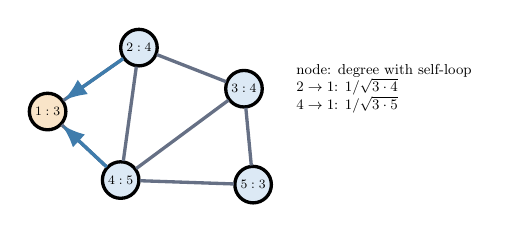
\begin{tikzpicture}[scale=0.58,transform shape]
    \examplegraph[fill=courselightorange]{$1:3$}{$2:4$}{$3:4$}{$4:5$}{$5:3$}
    \node[right=0.6cm of c,align=left,font=\small] {node: degree with self-loop\\$2\to1$: $1/\sqrt{3\cdot4}$\\$4\to1$: $1/\sqrt{3\cdot5}$};
    \draw[flow] (b)--(a); \draw[flow] (d)--(a);
  \end{tikzpicture}
  \end{center}
  \takeaway{So busy nodes do not dominate: each contribution is scaled down by how many neighbors both ends have.}
\end{frame}

\begin{frame}{GCN Layer and a Numeric Example\framecite{kipf2017}}
  \[
    \boxed{\mathbf h_v^{(k+1)}=\sigma\!\left(
      \sum_{u\in\widetilde{\mathcal N}(v)}
      \frac{1}{\sqrt{\widetilde d_v\widetilde d_u}}\,
      \mathbf W^{(k)}\mathbf h_u^{(k)}\right)}
  \]
  $\mathbf W^{(k)}$: learned weight matrix, the same for all nodes. $\sigma$: nonlinearity (for example ReLU).

  \smallskip
  Five-node graph, node 1: degrees with self-loops $\widetilde d_1=3$, $\widetilde d_2=4$, $\widetilde d_4=5$. Weights:
  \[
    \text{self: }\tfrac13\approx0.33,\quad
    \text{from }2:\tfrac1{\sqrt{12}}\approx0.29,\quad
    \text{from }4:\tfrac1{\sqrt{15}}\approx0.26.
  \]
  \takeaway{So GCN has fixed weights set by the graph's degrees; only $\mathbf W$ is learned. (Matrix form: appendix.)}
\end{frame}

\begin{frame}{GraphSAGE: Keep Self and Neighbors Separate\framecite{hamilton2017}}
  GraphSAGE averages the neighbors, then stacks the result next to the node's own state:
  \[
    \mathbf m_v=\frac{1}{|\mathcal N(v)|}\sum_{u\in\mathcal N(v)}\mathbf h_u,
    \qquad
    \boxed{\mathbf h_v^{(k+1)}=\sigma\!\left(\mathbf W^{(k)}[\mathbf h_v\,\|\,\mathbf m_v]\right)}.
  \]
  $[\cdot\,\|\,\cdot]$ is \emph{concatenation}: put two vectors one after the other.
  Example: $\mathbf h_v=(1,0)$ and $\mathbf m_v=(3,2)$ give $[\mathbf h_v\,\|\,\mathbf m_v]=(1,0,3,2)$, which $\mathbf W$ then mixes.
  \takeaway{So the layer can weigh ``what I am'' and ``what my neighbors look like'' differently.}
\end{frame}

\begin{frame}{GraphSAGE Works on Unseen Nodes\framecite{hamilton2017}}
  \begin{itemize}
    \item The learned weights act on features, not on stored node identities.
    \item So the same layer can embed a node, or even a whole graph, that was not in the training set (\emph{inductive} learning).
    \item For huge graphs one \emph{samples} a fixed number of neighbors per node, which saves computation at the cost of a noisier average.
  \end{itemize}
  \takeaway{So GraphSAGE suits graphs that grow or change, and large graphs where full neighborhoods are too costly.}
\end{frame}

\begin{frame}{Graph Attention: Learn the Neighbor Weights\framecite{velickovic2018}}
  GCN weights come from degrees. A \emph{graph attention network} (GAT) lets the model score each neighbor from the features:
  \[
    e_{vu}=a(\mathbf W\mathbf h_v,\mathbf W\mathbf h_u),\qquad
    \alpha_{vu}=\frac{\exp(e_{vu})}{\sum_{j\in\widetilde{\mathcal N}(v)}\exp(e_{vj})},
  \]
  \[
    \boxed{\mathbf h'_v=\sigma\!\Bigl(\sum_{u\in\widetilde{\mathcal N}(v)}\alpha_{vu}\mathbf W\mathbf h_u\Bigr)}.
  \]
  $a$ is a small learned scoring function, $e_{vu}$ the score of neighbor $u$ for node $v$,
  and softmax turns $v$'s scores into weights $\alpha_{vu}$ that add up to 1.
  Example: scores $(2,1,0)$ give weights $(0.67,\,0.24,\,0.09)$.
  \takeaway{So GAT decides from the features how much each neighbor counts, node by node.}
\end{frame}

\begin{frame}{Comparing the Three Layers}
  \begin{center}
  \footnotesize
  \begin{tabular}{@{}lll@{}}
    \textbf{Layer} & \textbf{How neighbors are weighted} & \textbf{Notable property}\\\hline
    GCN & fixed, from degrees & simple; undirected graphs\\
    GraphSAGE & plain mean, self kept apart & works on unseen nodes\\
    GAT & learned from features & weights depend on content
  \end{tabular}
  \end{center}
  Attention weights are a learned score, not automatically a causal explanation.
  \takeaway{So the three layers differ only in how they weight and combine neighbors; the message-passing skeleton is the same.}
\end{frame}



\section{Building Graph Models}
\sectiondivider{Building Graph Models}

\begin{frame}{Edge Features Belong Inside the Message}
  \[
    \boxed{\mathbf m_{uv}=M(\mathbf h_u,\mathbf h_v,\mathbf e_{uv})}.
  \]
  \begin{center}
  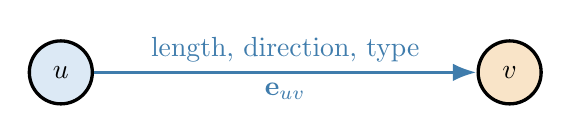
\begin{tikzpicture}[scale=0.95]
    \node[vertex] (u) at (1,0) {$u$};
    \node[vertex,fill=courselightorange] (v) at (7,0) {$v$};
    \draw[flow] (u)--node[above] {length, direction, type}node[below] {$\mathbf e_{uv}$}(v);
  \end{tikzpicture}
  \end{center}
  A relation can change what should be transmitted: a short stiff member and a long flexible one pass different information.
  In mechanics edge features are often a displacement, a distance or interface data.
  \takeaway{So whenever edges carry information, feed it into the message instead of discarding it.}
\end{frame}

\begin{frame}{A Global State or Virtual Node Shares Long-Range Context}
  \begin{center}
  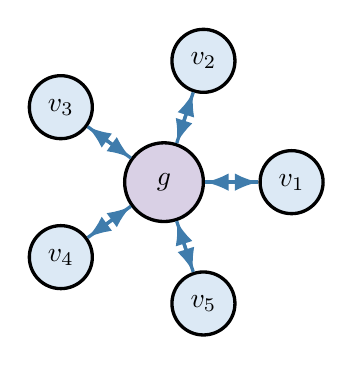
\begin{tikzpicture}[scale=0.6]
    \node[vertex,fill=coursepurple!28,minimum size=1.0cm] (g) at (5,0) {$g$};
    \foreach \i/\ang in {1/0,2/72,3/144,4/216,5/288}{
      \node[vertex] (n\i) at ($(g)+(\ang:2.7cm)$) {$v_{\i}$};
      \draw[flow] (n\i)--(g); \draw[flow] (g)--(n\i);
    }
  \end{tikzpicture}
  \end{center}
  A virtual node $g$ is connected to every node: it gathers from all of them and broadcasts back. A global feature (loading, temperature) can live there.
  \takeaway{So one extra node gives every node a shortcut to all others, at the price of a weaker locality bias.}
\end{frame}

\begin{frame}{Graph Readout Must Be Permutation Invariant}
  To predict for the whole graph, combine all node states $\mathbf h_v$ into one vector with a
  \emph{readout}: $\mathbf h_G=\operatorname{READOUT}(\{\mathbf h_v:v\in V\})$.
  Node states $(1,3),(2,0),(3,3)$ give:
  \[
    \text{sum}=(6,6),\qquad \text{mean}=(2,2),\qquad \text{max}=(3,3).
  \]
  \begin{itemize}
    \item Sum keeps counts and graph size; mean removes the effect of node count; max records whether a strong feature occurs anywhere.
  \end{itemize}
  \takeaway{So the readout choice encodes an assumption about the target, and all three ignore the node order.}
\end{frame}

\begin{frame}{A Batch Is a Disconnected Union of Graphs}
  \begin{center}
  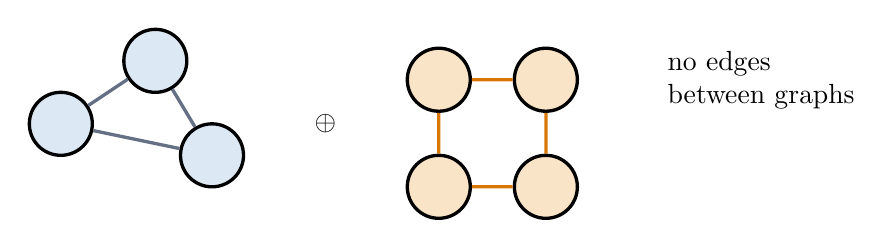
\begin{tikzpicture}[scale=0.8]
    \node[vertex] (a1) at (0,0) {}; \node[vertex] (a2) at (1.5,1) {};
    \node[vertex] (a3) at (2.4,-0.5) {};
    \draw[edge] (a1)--(a2)--(a3)--(a1);
    \node[vertex,fill=courselightorange] (b1) at (6,0.7) {};
    \node[vertex,fill=courselightorange] (b2) at (7.7,0.7) {};
    \node[vertex,fill=courselightorange] (b3) at (6,-1.0) {};
    \node[vertex,fill=courselightorange] (b4) at (7.7,-1.0) {};
    \draw[focus] (b1)--(b2)--(b4)--(b3)--(b1);
    \node at (4.2,0) {$\oplus$};
    \node[right=1.0cm of b2,align=left] {no edges\\between graphs};
  \end{tikzpicture}
  \end{center}
  Graphs have different sizes, so we train on several at once by placing them in one big graph with no edges between them:
  $\mathbf A_{\text{batch}}=\operatorname{blockdiag}(\mathbf A_1,\ldots,\mathbf A_B)$.
  A graph-membership vector tells the readout which nodes belong together.
  \takeaway{So message passing never mixes graphs, and the readout stays separate for each graph.}
\end{frame}

\begin{frame}{Meshes Need Geometrically Meaningful Relations}
  \begin{center}
  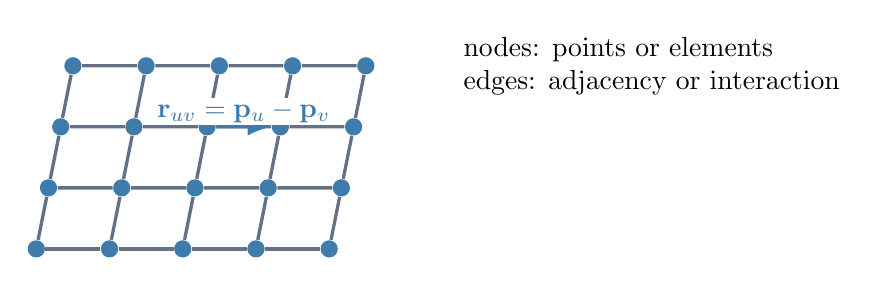
\begin{tikzpicture}[scale=0.62]
    \foreach \i in {0,...,4}{\foreach \j in {0,...,3}{
      \node[circle,fill=courseblue,inner sep=2.2pt] (n\i\j) at (1.5*\i+0.25*\j,1.25*\j) {};
    }}
    \foreach \i in {0,...,3}{\foreach \j in {0,...,3}{
      \pgfmathtruncatemacro{\next}{\i+1}\draw[edge] (n\i\j)--(n\next\j);
    }}
    \foreach \i in {0,...,4}{\foreach \j in {0,...,2}{
      \pgfmathtruncatemacro{\next}{\j+1}\draw[edge] (n\i\j)--(n\i\next);
    }}
    \draw[flow] (n22)--node[above,fill=white,inner sep=1pt] {$\mathbf r_{uv}=\mathbf p_u-\mathbf p_v$}(n32);
    \node[right=1.0cm of n43,align=left] {nodes: points or elements\\edges: adjacency or interaction};
  \end{tikzpicture}
  \end{center}
  The edge feature $\mathbf r_{uv}$ is the relative position of two nodes ($\mathbf p_u$ is the position of node $u$).
  Relative positions do not change if the whole mesh is shifted; distances also survive rotations, while vectors rotate with the mesh.
  \takeaway{So choose edge features that carry the symmetry the physics has, such as shift or rotation invariance.}
\end{frame}

\begin{frame}{Graph Construction Is Part of the Model}
  \begin{itemize}
    \item Which entities become nodes?
    \item Which relations become edges: topology, radius, or nearest neighbors?
    \item Are edges directed, weighted, typed, or time dependent?
    \item Which attributes belong on nodes, edges, or the whole graph?
  \end{itemize}
  \begin{center}
  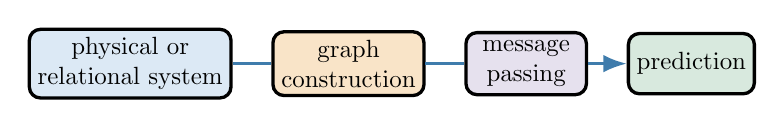
\begin{tikzpicture}[node distance=0.55cm,scale=0.9,transform shape]
    \node[box,fill=courselightblue] (system) {physical or\\relational system};
    \node[box,fill=courselightorange,right=of system] (graph) {graph\\construction};
    \node[box,fill=coursepurple!18,right=of graph] (gnn) {message\\passing};
    \node[box,fill=coursegreen!18,right=of gnn] (prediction) {prediction};
    \draw[flow] (system)--(graph)--(gnn)--(prediction);
  \end{tikzpicture}
  \end{center}
  \takeaway{So a GNN cannot recover relations that the graph construction removed; design the graph deliberately.}
\end{frame}



\section{Limits of Message Passing}
\sectiondivider{Limits of Message Passing}

\begin{frame}{Oversmoothing: Repeated Averaging Blurs the Nodes}
  Each layer averages a node with its neighbors, which is a smoothing step. What happens after many layers?
  We test it on the five-node graph with starting values $(3,1,-1,2,-3)$ and pure averaging
  (each step: replace a value by the mean of itself and its neighbors; no learning, no nonlinearity).
  \begin{center}
  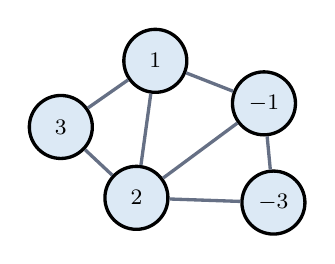
\begin{tikzpicture}[scale=0.6]
    \examplegraph{$3$}{$1$}{$-1$}{$2$}{$-3$}
  \end{tikzpicture}
  \end{center}
  \takeaway{So the question is whether the nodes stay distinguishable after many averaging steps.}
\end{frame}

\begin{frame}{Oversmoothing: The Computed Result}
  \begin{center}
  \begin{tikzpicture}
    \begin{axis}[width=0.82\textwidth,height=5.2cm,xlabel={averaging steps $k$},ylabel={node value},
      xmin=0,xmax=10,legend style={font=\scriptsize,at={(1.02,0.5)},anchor=west},
      tick label style={font=\scriptsize},label style={font=\small},grid=major,grid style={gray!20}]
      \addplot[very thick,color=courseblue] table[x=k,y=n1] {assets/generated/oversmoothing.dat};
      \addlegendentry{node 1}
      \addplot[very thick,color=courseorange] table[x=k,y=n2] {assets/generated/oversmoothing.dat};
      \addlegendentry{node 2}
      \addplot[very thick,color=coursegreen] table[x=k,y=n3] {assets/generated/oversmoothing.dat};
      \addlegendentry{node 3}
      \addplot[very thick,color=coursepurple] table[x=k,y=n4] {assets/generated/oversmoothing.dat};
      \addlegendentry{node 4}
      \addplot[very thick,color=coursered] table[x=k,y=n5] {assets/generated/oversmoothing.dat};
      \addlegendentry{node 5}
    \end{axis}
  \end{tikzpicture}
  \end{center}
  {\small Spread (max minus min): $6.0$ at $k=0$, $0.34$ at $k=4$, $0.005$ at $k=10$.}
  \takeaway{So with averaging alone all nodes converge to nearly the same value; deep stacks risk losing the differences between nodes.}
\end{frame}

\begin{frame}{Two More Limits}
  \begin{columns}[T]
    \begin{column}{0.48\textwidth}
      \textbf{Oversquashing}
      \[
        \text{many signals}
        \longrightarrow \mathbf h_v\in\mathbb R^d
      \]
      Fixed-width states and few connecting edges form a bottleneck.

      Virtual nodes or better connectivity can shorten paths.
    \end{column}
    \begin{column}{0.48\textwidth}
      \textbf{Expressiveness}\framecite{xu2019}
      \[
        \begin{gathered}G\not\cong H\quad\text{can still yield}\\
        f(G)=f(H).\end{gathered}
      \]
      With matching initial features, graphs indistinguishable to the
      1-Weisfeiler--Lehman test remain indistinguishable to standard message passing.

      Richer features or more expressive layers may help.
    \end{column}
  \end{columns}
  \takeaway{More depth increases reach; it does not remove bottlenecks or guarantee distinguishability.}
\end{frame}



\appendix
\sectiondivider{Appendix: optional depth}

\begin{frame}{Appendix: Message Passing Is Permutation Equivariant}
  Relabel nodes by a bijection $\pi$. The neighborhoods become
  $\mathcal N'(\pi(v))=\{\pi(u):u\in\mathcal N(v)\}$.
  Shared messages and symmetric aggregation give
  \[
    \mathbf m'_{\pi(v)}
    =\operatorname{AGG}\{\mathbf m'_{\pi(u)\pi(v)}\}
    =\operatorname{AGG}\{\mathbf m_{uv}\}=\mathbf m_v .
  \]
  Therefore the shared update gives
  \[
    \boxed{\mathbf h'^{(k+1)}_{\pi(v)}=\mathbf h^{(k+1)}_v}.
  \]
  Composing equivariant layers preserves equivariance.
\end{frame}

\begin{frame}{Appendix: The Weisfeiler--Lehman Limit\framecite{xu2019}}
  The 1-WL test colors each node $v$ with $c_v$ and refreshes the colors repeatedly,
  where $\operatorname{HASH}$ maps its input to a new color (same input, same color):
  \[
    c_v^{(k+1)}=\operatorname{HASH}\!\left(
      c_v^{(k)},\{c_u^{(k)}:u\in\mathcal N(v)\}\right),
  \]
  \[
    \mathbf h_v^{(k+1)}=U\!\left(\mathbf h_v^{(k)},
      \operatorname{AGG}\{\mathbf h_u^{(k)}:u\in\mathcal N(v)\}\right).
  \]
  \begin{itemize}
    \item Standard message-passing GNNs cannot distinguish graphs that 1-WL cannot.
    \item Injective multiset aggregation can match 1-WL distinguishing power.
    \item Mean or max aggregation may merge different multisets earlier.
  \end{itemize}
\end{frame}

\begin{frame}{Appendix: Oversquashing}
  \begin{center}
  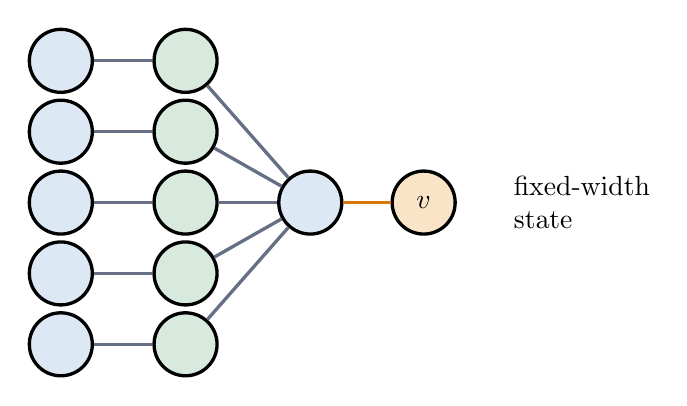
\begin{tikzpicture}[scale=0.72]
    \node[vertex,fill=courselightorange] (v) at (7,0) {$v$};
    \node[vertex] (a) at (5,0) {}; \draw[focus] (a)--(v);
    \foreach \i/\y in {1/2.5,2/1.25,3/0,4/-1.25,5/-2.5}{
      \node[vertex,fill=coursegreen!18] (b\i) at (2.8,\y) {};
      \draw[edge] (b\i)--(a);
      \node[vertex,fill=courselightblue] (c\i) at (0.6,\y) {};
      \draw[edge] (c\i)--(b\i);
    }
    \node[right=0.6cm of v,align=left] {fixed-width\\state};
  \end{tikzpicture}
  \end{center}
  \begin{itemize}
    \item The number of distant sources can grow faster than the state dimension.
    \item A narrow bottleneck forces many signals through few edges.
    \item More layers increase reach but do not remove the compression.
  \end{itemize}
\end{frame}

\begin{frame}{Appendix: GCN in Matrix Form and Linear Smoothing}
  With adjacency $\mathbf A$, $\widetilde{\mathbf A}=\mathbf A+\mathbf I$ and the diagonal degree matrix
  $\widetilde{\mathbf D}_{vv}=\sum_u\widetilde A_{vu}$, one GCN layer for all nodes at once is
  \[
    \mathbf H^{(k+1)}=\sigma\!\left(
      \widetilde{\mathbf D}^{-1/2}\widetilde{\mathbf A}\widetilde{\mathbf D}^{-1/2}
      \mathbf H^{(k)}\mathbf W^{(k)}\right),
  \]
  where row $v$ of $\mathbf H^{(k)}$ is $\mathbf h_v^{(k)}$. This form assumes an undirected graph.
  Dropping $\sigma$ and $\mathbf W$, $K$ layers apply $\mathbf S^K$ with
  $\mathbf S=\widetilde{\mathbf D}^{-1/2}\widetilde{\mathbf A}\widetilde{\mathbf D}^{-1/2}$,
  whose repeated powers are dominated by low-frequency graph modes: the linear picture of oversmoothing.
\end{frame}

\end{document}
